\documentclass[a4paper, oneside, openany, dvipsnames, table]{article}
\usepackage{../../template/SWEightStyle}
\usepackage{ltablex}
\usepackage{tabularx}
\usepackage{pdfpages}
\usepackage{svg}
\usepackage{eurosym}


\setcounter{secnumdepth}{3}


\newcommand{\Titolo}{Manuale Utente}

\newcommand{\Gruppo}{SWEight}

\newcommand{\Approvatore}{Damien Ciagola}
\newcommand{\Redattori}{Alberto Bacco \newline Sebastiano Caccaro \newline Gheorghe Isachi \newline Gionata Legrottaglie}
\newcommand{\Verificatori}{Francesco Corti \newline Francesco Magarotto}

\newcommand{\pathimg}{../template/img/logoSWEight.png}

\newcommand{\Versionedoc}{1.0.0}

\newcommand{\Distribuzione}{\proponente \newline Prof. Vardanega Tullio \newline Prof. Cardin Riccardo \newline Gruppo SWEight}

\newcommand{\Uso}{Esterno}

\newcommand{\NomeProgetto}{Colletta}

\newcommand{\Mail}{SWEightGroup@gmail.com}

\newcommand{\DescrizioneDoc}{Questo documento si occupa di fornire le modalità di utilizzo del software Colletta commissionato}


\begin{document}
\copertina{}

\definecolor{greySWEight}{RGB}{255, 71, 87}
\definecolor{greyROwSWEight}{RGB}{234, 234, 234}

\section*{Registro delle modifiche}
{
	\rowcolors{2}{greyROwSWEight}{white}
	\renewcommand{\arraystretch}{1.5}
	\centering
	\begin{longtable}{ c c C{4cm}  c  c }
		
		\rowcolor{greySWEight}
		\textcolor{white}{\textbf{Versione}} & \textcolor{white}{\textbf{Data}} & \textcolor{white}{\textbf{Descrizione}} & \textcolor{white}{\textbf{Nominativo}} & \textcolor{white}{\textbf{Ruolo}}\\
		1.2.2 & 2019-02-25 & Ampliamento sezione 5.4 e 3.2.5.2 & Alberto Bacco & \reda{} \\
		
		1.2.1 & 2019-02-23 & Aggiunta sezione 3.2.5.8 Checkstyle & Sebastiano Caccaro & \reda{} \\		
		
		1.2.0 & 2019-02-20 & Aggiunta scelte tecnologiche 3.2.4.2, da 3.4.5.4 a 3.4.5.7, 4.3.1.4, 4.3.2.2, 4.4.6 e figlie & Sebastiano Caccaro & \reda{} \\	
		
		1.1.5 & 2019-02-20 & Modifica sezione 2 & Alberto Bacco & \reda{} \\
		
		1.1.4 & 2019-02-18 & Correzione errori grammatica, spostate sottosezioni di asana da 4.3 a 5.2, & Alberto Bacco & \reda{} \\
		
		1.1.3 & 2019-02-14 & Riorganizzazione e correzione errori sezione 5 & Enrico Muraro & \reda{} \\
		
		1.1.2 & 2019-02-03 & Modifica sottosezione 4.1.10, 4.3.1.4, 4.3.1.5, 4.3.1.6 & Alberto Bacco& \reda{} \\	
		
		1.1.1 & 2019-01-31 & Modifica struttura e contenuti sezione 3  & Damien Ciagola & \reda{} \\	
		
		1.1.0 & 2019-01-27 & Sezione Qualità 4.2 & Sebastiano Caccaro & \reda{} \\	
		
		1.0.1 & 2019-01-25 & Parziale ristrutturazione della struttura del documento & Sebastiano Caccaro & \reda{} \\		
		
		1.0.0 & 2019-01-11 & Approvazione per il rilascio & Sebastiano Caccaro & \Res{} \\
		
		0.9.0 & 2019-01-9 & Verifica finale & Francesco Corti & \ver{} \\
		
		0.9.0 & 2019-01-8 & Aggiunta lista di controllo & Gionata Legrottaglie & \reda{} \\
		
		0.8.0 & 2018-12-23 & Correzioni errori ortografici & Gionata Legrottaglie & \reda{} \\
		
		0.7.0 & 2018-12-20 & Verifica documento & Francesco Corti & \ver{}\\
		
		0.6.0 & 2018-12-18 & Aggiunta sottosezione 5.2.2.2, 5.2.2.3, 5.2.2.4 & Francesco Magarotto & \reda{} \\
		
		0.5.2 & 2018-12-16 & Modifica sezione 4.1.5.3 & Alberto Bacco & \reda{} \\
		
		0.5.2 & 2018-12-16 & Modifica sezione 4.1.5.3 & Alberto Bacco & \reda{} \\
		
		0.5.2 & 2018-12-16 & Aggiunte sottosezioni  & Alberto Bacco & \reda{} \\
		
		0.5.1 & 2018-12-15 & Aggiunte sottosezioni 5.3, 5.4, 5.5, 5.6, 5.7, 5.8 & Alberto Bacco & \reda{} \\
		
		0.5.0 & 2018-12-15 & Aggiunta sezione 5 e sottosezioni 5.1, 5.2 & Gionata Legrottaglie & \reda{} \\
		
		0.4.1 & 2018-12-11 & Aggiunta sezione 4.1.7.3.1 & Francesco Magarotto & \reda{} \\ 
		
		0.4.0 & 2018-12-10 & Aggiunte sottosezioni 4.1.5, 4.1.6, 4.1.7, 4.1.8 & Gionata Legrottaglie & \reda{} \\ 
		0.4.0 & 2018-12-09 & Aggiunta sezione 4 e sottosezioni 4.1.1, 4.1.2, 4.1.3, 4.1.4 & Gionata Legrottaglie & \reda{} \\ 
		
		0.3.1 & 2018-12-07 & Aggiunta sottosezione 3.2 & Gionata Legrottaglie & \reda{} \\ 
		
		0.3.0 & 2018-12-06 & Aggiunta sezione 3 e sottosezione 3.1 & Gionata Legrottaglie & \reda{} \\ 
		
		0.2.0 & 2018-12-05 & Aggiunti i riferimenti & Gionata Legrottaglie & \reda{} \\ 
		
		0.1.0 & 2018-11-30 & Aggiunta introduzione & Gionata Legrottaglie & \reda{} \\
		
		0.0.1 & 2018-11-28 & Creazione scheletro del documento & Gionata Legrottaglie & \reda{}\\
		
	\end{longtable}

}
\newpage
\tableofcontents
\newpage

\section{Introduzione}
	\subsection{Scopo del documento}
		% vecchia introduzione
% In questo documento è illustrata la {strategia}\ped{G} di {verifica}\ped{G} e 
% {validazione}\ped{G} del gruppo \gruppo . Tale strategia è fondamentale per dare una 
% misurazione oggettiva e quantificabile del livello di {qualità}\ped{G} di quanto viene 
% prodotto. \newline
% Ciò è vantaggioso sia per il gruppo \gruppo , che può facilmente individuare difetti 
% durante lo svolgimento del progetto, sia per il {committente}\ped{G}, che può costantemente 
% monitorare la qualità del prodotto in base a criteri oggettivi e prestabiliti.

% alternativa alla prima introduzione
In questo documento sono illustrate le {strategie}\ped{G} di {verifica}\ped{G}e 
{validazione}\ped{G} del gruppo \gruppo. 
Tale strategia ci si assicura la qualità dei processi, dei documenti e delle procedure 
utilizzate per gestire e sviluppare i risultati finali.
Lo scopo di questo documento è descrivere le informazioni necessarie per gestire efficacemente 
la qualità del progetto, dalla pianificazione alla consegna, comprendendo obiettivi 
di qualità, responsabilità, e l'approccio di gestione della qualità per 
garantire che gli obiettivi siano raggiunti.\newline
Ciò è vantaggioso sia per il gruppo \gruppo , che può facilmente individuare difetti 
durante lo svolgimento del progetto, sia per il {committente}\ped{G}, che può costantemente 
monitorare la qualità del prodotto in base a criteri oggettivi e prestabiliti.


	\subsection{Scopo del prodotto}
		Il progetto prevede la realizzazione di una piattaforma collaborativa di raccolta dati in cui gli utenti possano predisporre e/o svolgere piccoli esercizi di analisi grammaticale. Lo scopo è raccogliere dati relativi sia  agli esercizi predisposti, che al loro svolgimento da parte degli utenti. Sviluppatori e ricercatori utilizzeranno queste informazione per insegnare ad un elaboratore a svolgere i medesimi esercizi, mediante tecniche di apprendimento automatico.

%Questa parte è un copia-incolla cafonissimo dal capitolato della mivoc
%Siccome è proprio quello che vogliono, non mi sembrava il caso di andare a modifcarla
	\subsection{Glossario}
		
\section*{F}
\textbf{Freeling}: the library for pos-tagging developed by TALP Research Center written in C++;
\section*{P}
\textbf{Pos-tagging}: part-of-speech tagging, also called grammatical tagging or word-category disambiguation, is the process of marking up a word in a text (corpus) as corresponding to a particular part of speech; \\ 
\textbf{POJO}: Plain Old Java Object, is an ordinary Java object, not bound by any special restriction and not requiring any class path. In Spring it refers to a Java object (instance of definition) that isn't bogged down by framework extensions;
\section*{J}
\textbf{JSON}: JavaScript Object Notation, is a lightweight data-interchange format.  It is easy for humans to read and write. It is easy for machines to parse and generate.\\
\textbf{JWT}: JSON Web Token, a JSON-based open standard (RFC 7519) for creating access tokens that assert some number of claims;

	\subsection{Riferimenti}
		\subsubsection{Riferimenti normativi}
			\begin{itemize}
	\item \textbf{Norme di Progetto:} \NdP ;
	\item \textbf{Capitolato d'appalto C2: } Colletta \newline
		  \url{https://www.math.unipd.it/~tullio/IS-1/2018/Progetto/C2.pdf}.
\end{itemize}
		\subsubsection{Riferimenti informativi}
			\begin{itemize}
    \item Software Engineering (10th edition) - Ian Sommerville
    \item Slide "Gestione di Progetto", corso di Ingegneria del Software
          \newline \url{https://www.math.unipd.it/~tullio/IS-1/2018/Dispense/L06.pdf}
\end{itemize}
	\subsection{Scadenze}
		Il gruppo \gruppo\space si imppegna a rispettare le seguenti scadenze, sulle quali
è basata la pianficazione del progetto.

\rowcolors{2}{greyROwSWEight}{white}
\renewcommand{\arraystretch}{1.5}
\begin{table}[H]	
	\begin{center}
	    \begin{tabular}{| c | c | }
	        \hline
	        \rowcolor{greySWEight}
	        \textcolor{white}{\textbf{Revisione}} & \textcolor{white}{\textbf{Scadenza}}\\
	        RR & 21/01/2019 \\
	        RP & 15/03/2019 \\
	        RQ & 19/04/2019 \\
	        RA & 17/05/2019 \\
	        \hline
	    \end{tabular}
	    \caption{Scadenze} \label{tab:tabellascadenze} 
	\end{center}
\end{table}

   
\newpage
\section{Analisi dei rischi}
	\subsection{Document goal}
The purpose of this document is to provide all the necessary information to extend, correct and improve Colletta.
There will be additional information regarding setting up the development environment to work in an environment that is as consistent as possible with that used
by the other members of group SWEight, but can be ignored if you only want to use part of the product.
This guide was written taking into account the Microsoft Windows and Linux operating systems. If other systems are used, compatibility issues may arise, even if it's unlikely. In this case refer to the git page. This document will grow as the product will be fully
developed.

\subsection{Product goal}
The purpose of the product is the creation of a collaborative data collection platform where users can prepare and/or perform small grammar exercises. 
The front-end of the system consists of a web application developed with React and Redux, while the back-end is a Spring Boot application written in Java, which will handle HTTP Requests sent from the front-end. 

\subsection{References}


\subsubsection{Installation references}

\begin{itemize}
\item \textbf{Git}: \url{https://git-scm.com/}
\item \textbf{Node.js}: \url{https://nodejs.org/en/}
\item \textbf{NPM}: \url{https://www.npmjs.com/}
\item \textbf{Oracle JDK}: \url{https://www.oracle.com/technetwork/java/javase/downloads/index.html}
\item \textbf{OpenJDK}: \url{https://openjdk.java.net/}
\item \textbf{Maven}: \url{https://maven.apache.org/}
\item \textbf{Lombok}: \url{https://projectlombok.org/}
\item \textbf{VSCode}: \url{https://code.visualstudio.com/} 

\end{itemize}

\subsubsection{Legal references}
\begin{itemize}
\item \textbf{MIT License}: \url{https://opensource.org/licenses/MIT}
\end{itemize}

%\subsubsection{Informative references}

	\newcommand{\barra}{\hline \hline \hline}
\renewcommand{\arraystretch}{1.5}
\def\tabularxcolumn#1{m{#1}}
\begin{tabularx}{\textwidth}{C{0.2\textwidth} X C{0.2\textwidth}}
\hline
\rowcolor{greySWEight}
    \textcolor{white}{\textbf{Nome}} & \textcolor{white}{\textbf{Descrizione}}&
    \textcolor{white}{\textbf{Livello di Rischio}}\endhead
\hline
 \textbf  	
 	{Conflitti fra i membri del gruppo}&
    Per molti membri del gruppo questa è la prima esperienza di lavoro in gruppo con un certo
    numero di persone.Ciò potrebbe causare inconvenienti di natura interpersonale.&
    
    Probabilità: \newline \textbf{Bassa}\newline
    Gravità: \newline \textbf{Alta}\\
    
    Contromisure &
    \multicolumn{2}{L{\dimexpr\textwidth-4\tabcolsep-0.2\textwidth}}{
    Ogni problema andrà tempestivamente riportato al responsabile. Ove non sia possibile
    trovare una soluzione, il responsabile cercherà di assegnare ruoli e attività che 
    minimizzino l'interazione fra i membri in causa.
    }\\
    \barra
    
    
 
 \textbf
 	{Assenza prolungata di un membro del gruppo}&
    \'E possibile che, a causa di problemi di salute o familiari, un membro del gruppo possa
    non poter svolgere le sue mansioni per un certo periodo di tempo. &
    Probabilità: \newline \textbf{Bassa}\newline
    Gravità: \newline \textbf{Alta}\\
    
    Contromisure&
    \multicolumn{2}{L{\dimexpr\textwidth-4\tabcolsep-0.2\textwidth}}{
    A seconda della natura del problema e delle attività lasciate in sospeso, il responsabile
    può ridistribuire il carico di lavoro del membro assente o posticiparle e rivedere
    la pianificazione
    }\\
    \barra

\textbf
    {Incompatibilità orari dei membri del gruppo}&
   A causa di ubicazione geografica e diversi impegni universitari e lavorativi
   dei vari membri del gruppo, può essere complicato incontrarsi di persona per
   discutere del progetto.&
   Probabilità: \newline \textbf{Alta}\newline
   Gravità: \newline \textbf{Bassa}\\
   
   Contromisure&
   \multicolumn{2}{L{\dimexpr\textwidth-4\tabcolsep-0.2\textwidth}}{
   Creazione di una tabella oraria con gli impegni di ogni membro del gruppo. \newline
   Ogni riunione avrà uno scopo ben preciso, e ogni membro è tenuto a preparasi
   attentamente per sfruttare al meglio il tempo disponibile. \newline
   In caso non sia possibile organizzare un incontro fisico, è sempre possibile
   discutere in videoconferenza.
   Una riunione può essere svolta anche in assenza 2 membri.
   }\\
   \barra
   
\textbf
    {Incompatibilità orari dei membri del gruppo}&
   A causa di ubicazione geografica e diversi impegni universitari e lavorativi
   dei vari membri del gruppo, può essere complicato incontrarsi di persona per
   discutere del progetto.&
   Probabilità: \newline \textbf{Alta}\newline
   Gravità: \newline \textbf{Bassa}\\
   
   Contromisure&
   \multicolumn{2}{L{\dimexpr\textwidth-4\tabcolsep-0.2\textwidth}}{    
   Creazione di una tabella oraria con gli impegni di ogni membro del gruppo. \newline
   Ogni riunione avrà uno scopo ben preciso, e ogni membro è tenuto a preparasi
   attentamente per sfruttare al meglio il tempo disponibile. \newline
   In caso non sia possibile organizzare un incontro fisico, è sempre possibile
   discutere in videoconferenza.
   Una riunione può essere svolta anche in assenza 2 membri.
   }\\
   \barra
   
\textbf
    {Inesperienza tecnologica}&
   Alcuni membri del gruppo potrebbero non conoscere alcune delle tecnologie utilizzate nel
   progetto&
   Probabilità: \newline \textbf{Alta}\newline
   Gravità: \newline \textbf{Media}\\
   
   Contromisure&
   \multicolumn{2}{L{\dimexpr\textwidth-4\tabcolsep-0.2\textwidth}}{    
   Studio individuale delle tecnologie sconosciute, eventualmente coadiuvato da un membro più
   esperto in una determinata tecnologia. L'assegnazione delle attività deve tenere conto delle
   conoscenze tecnologiche degli assegnatari.
   }\\
   \barra
   
   	{Danni hardware e software}&
   Possibili malfunzionamenti agli strumenti di lavoro possono rallentare lo svolgimento delle attività o
   causare la perdita di lavoro già svolto.
   &
   Probabilità: \newline \textbf{Bassa}\newline
   Gravità: \newline \textbf{Media}\\
   
   Contromisure&
   \multicolumn{2}{L{\dimexpr\textwidth-4\tabcolsep-0.2\textwidth}}{    
   Ogni incremento significativo nello svolgimento di un'attività va tempestivamente versionato nel cloud.
 
   }\\
   \barra

   {Inesperienza organizzativa}&
   Nessuno dei membri del team ha mai lavorato ad un progetto con questo livello di organizzazione.
   Pertanto, può risultare difficile stimare il costo temporale delle attività e organizzare quest'ultime
   nel tempo.
   &
   Probabilità: \newline \textbf{Alta}\newline
   Gravità: \newline \textbf{Media}\\
   
   Contromisure&
   \multicolumn{2}{L{\dimexpr\textwidth-4\tabcolsep-0.2\textwidth}}{    
   Ogni attività è comprensiva di un periodo di slack. Pianificare milestone più frequenti durante le prime
   fasi del progetto, in modo da limitare il margine di errore e da correggere il tiro con i consuntivi.
 
   }\\
   \barra
\caption{Analisi dei rischi} \label{tab:sometab} 
\end{tabularx}




\newpage
\section{Modelli di sviluppo}
	\subsection{Document goal}
The purpose of this document is to provide all the necessary information to extend, correct and improve Colletta.
There will be additional information regarding setting up the development environment to work in an environment that is as consistent as possible with that used
by the other members of group SWEight, but can be ignored if you only want to use part of the product.
This guide was written taking into account the Microsoft Windows and Linux operating systems. If other systems are used, compatibility issues may arise, even if it's unlikely. In this case refer to the git page. This document will grow as the product will be fully
developed.

\subsection{Product goal}
The purpose of the product is the creation of a collaborative data collection platform where users can prepare and/or perform small grammar exercises. 
The front-end of the system consists of a web application developed with React and Redux, while the back-end is a Spring Boot application written in Java, which will handle HTTP Requests sent from the front-end. 

\subsection{References}


\subsubsection{Installation references}

\begin{itemize}
\item \textbf{Git}: \url{https://git-scm.com/}
\item \textbf{Node.js}: \url{https://nodejs.org/en/}
\item \textbf{NPM}: \url{https://www.npmjs.com/}
\item \textbf{Oracle JDK}: \url{https://www.oracle.com/technetwork/java/javase/downloads/index.html}
\item \textbf{OpenJDK}: \url{https://openjdk.java.net/}
\item \textbf{Maven}: \url{https://maven.apache.org/}
\item \textbf{Lombok}: \url{https://projectlombok.org/}
\item \textbf{VSCode}: \url{https://code.visualstudio.com/} 

\end{itemize}

\subsubsection{Legal references}
\begin{itemize}
\item \textbf{MIT License}: \url{https://opensource.org/licenses/MIT}
\end{itemize}

%\subsubsection{Informative references}

	\subsection{Motivazioni}
		L'analisi dei rischi ha stimato un basso rischio di cambio dei requisiti da parte della proponente.
Ciò significa che è possibile adottare un modello di sviluppo che prevede un'approfondita fase di 
analisi e progettazione iniziale.
La scelta è quindi ricaduta sul modello di sviluppo incrementale, che, inoltre, presenta altre
caratteristiche congeniali alle intenzioni del gruppo \gruppo \space :
\begin{itemize}
    \item Lo sviluppo del prodotto software è diviso in varie attività singole, comportando i seguenti vantaggi:
    \begin{itemize}
    	\item Maggior semplicità dello sviluppo di un'attività
    	\item Maggior semplicità in fase di test e troubleshooting
    	\item Migliore parallelizzazione del lavoro
    	\item Minore probabilità di incorrere in ritardi
    	\item Maggiore facilità nel rilascio
    \end{itemize}
    \item Le suddette attività sono ordinate in ordine di importanza, e vengono sviluppati prima i requisti di maggiore rilevanza per il committente
    \item Creazione di milestone per suddividere meglio il lavoro e per ottenere riscontri dal committente sul soddisfacimento dei requisiti
\end{itemize}
\newpage
\section{Pianificazione}
	\subsection{Document goal}
The purpose of this document is to provide all the necessary information to extend, correct and improve Colletta.
There will be additional information regarding setting up the development environment to work in an environment that is as consistent as possible with that used
by the other members of group SWEight, but can be ignored if you only want to use part of the product.
This guide was written taking into account the Microsoft Windows and Linux operating systems. If other systems are used, compatibility issues may arise, even if it's unlikely. In this case refer to the git page. This document will grow as the product will be fully
developed.

\subsection{Product goal}
The purpose of the product is the creation of a collaborative data collection platform where users can prepare and/or perform small grammar exercises. 
The front-end of the system consists of a web application developed with React and Redux, while the back-end is a Spring Boot application written in Java, which will handle HTTP Requests sent from the front-end. 

\subsection{References}


\subsubsection{Installation references}

\begin{itemize}
\item \textbf{Git}: \url{https://git-scm.com/}
\item \textbf{Node.js}: \url{https://nodejs.org/en/}
\item \textbf{NPM}: \url{https://www.npmjs.com/}
\item \textbf{Oracle JDK}: \url{https://www.oracle.com/technetwork/java/javase/downloads/index.html}
\item \textbf{OpenJDK}: \url{https://openjdk.java.net/}
\item \textbf{Maven}: \url{https://maven.apache.org/}
\item \textbf{Lombok}: \url{https://projectlombok.org/}
\item \textbf{VSCode}: \url{https://code.visualstudio.com/} 

\end{itemize}

\subsubsection{Legal references}
\begin{itemize}
\item \textbf{MIT License}: \url{https://opensource.org/licenses/MIT}
\end{itemize}

%\subsubsection{Informative references}

	\subsection{Analisi}
		Nella seguente tabella è illustrato il consuntivo del periodo di Analisi.

\begin{table}[H]
\centering
\begin{tabular}{c|ccc|ccc}
\rowcolor{greySWEight}
\multicolumn{1}{c}{} & \multicolumn{3}{c}{\textcolor{white}{\textbf{Ore}}} & \multicolumn{3}{c}{\textcolor{white}{\textbf{Costo in Euro}}} \\
{\textbf{Ruolo}} & {\textbf{Preventivo}} & {\textbf{Consuntivo}} & {\textbf{Delta}} & {\textbf{Preventivo}} & {\textbf{Consuntivo}} & {\textbf{Delta}} \\
Responsabile & 20 & 24 & +4 &  600,00 &  720,00 & + 120,00 \\
Amministratore & 20 & 22 & +2 &  400,00 &  440,00 & + 40,00 \\
Analista & 70 & 74 & +4 &  1.750,00 &  1.850,00 & + 100,00 \\
Progettista & 0 & 0 & 0 &  0,00 &  0,00 &  0,00 \\
Programmatore & 0 & 0 & 0 &  0,00 &  0,00 &  0,00 \\
Verificatore & 50 & 46 & -4 &  750,00 &  690,00 & - 60,00 \\
\hline
\textbf{Totale} & \textbf{160} & \textbf{166} & \textbf{+6} &  \textbf{3.500,00} &  \textbf{3.700,00} & \textbf{+ 200,00} \\


\end{tabular}
\caption{Consuntivo del periodo di Analisi}
\end{table}
	
	\subsection{Consolidamento}
		\subsubsection{Prospetto Orario}
Di seguito è riportata la suddivisione oraria dei ruoli nel periodo di Consolidamento.




\begin{table}[H]	
	\begin{center}
	    \begin{tabular}{cccccccc}
	  		
			\rowcolor{greySWEight}
			\textcolor{white}{\textbf{Nome}} & \textcolor{white}{\textbf{Re}} & \textcolor{white}{\textbf{Am}} & \textcolor{white}{\textbf{An}} & \textcolor{white}{\textbf{Pj}} & \textcolor{white}{\textbf{Pr}} & \textcolor{white}{\textbf{Ve}} & \textcolor{white}{\textbf{Totale}}
			\\ \hline
			Bacco Alberto & 5 & & & & & & 5 \\
			Caccaro Sebastiano & & & & & & 5 & 5 \\
			Ciagola Damien & & 5 & & & & & 5 \\
			Corti Francesco & & & & & & 5 & 5 \\
			Isachi Gheorghe & & 5 & & & & & 5 \\
			Legrottagle Gionata & & & 5 & & & & 5 \\
			Magarotto Francesco & & & & & & 5 & 5 \\
			Muraro Enrico & & & & & & 5 & 5 \\

			\end{tabular}
	    \caption{Tabella della suddivisione oraria dei membri del gruppo nel periodo di Consolidamento} \label{tab:tabellaPersoneConsolidamento} 
	\end{center}
\end{table}

La tabella della suddivisione oraria è rappresentata nel seguente grafico.
\begin{figure}[H]
	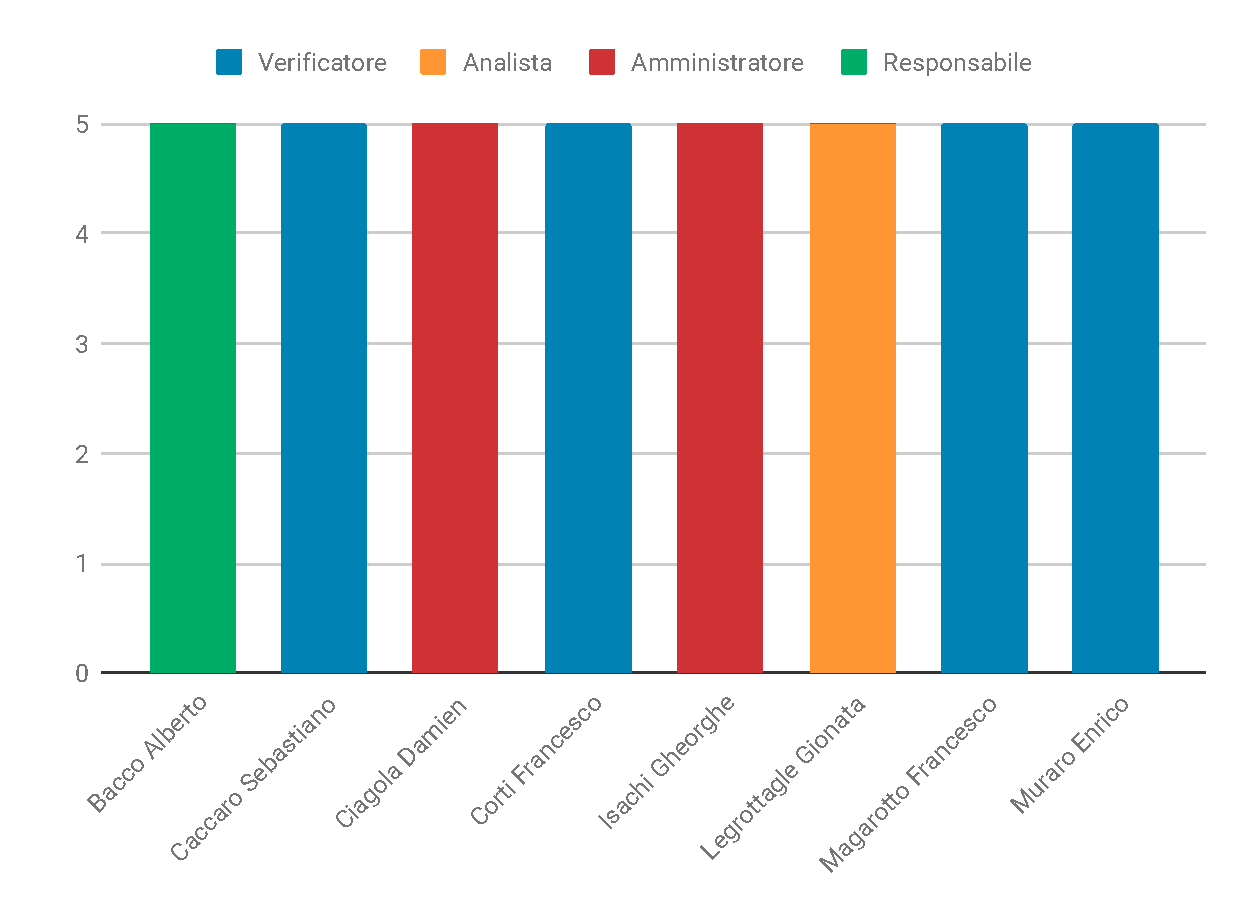
\includegraphics[width=1\linewidth]{Preventivo/grafici/CO1.pdf}
	\caption{Grafico della suddivisione oraria dei membri del gruppo nel periodo di Consolidamento}
\end{figure}

\subsubsection{Prospetto Economico}
Nella seguente tabella sono riportate le ore e i costi preventivati per ogni ruolo durante la fase di Consolidamento.


\begin{table}[H]	
	\begin{center}
	    \begin{tabular}{C{4cm}C{1cm}C{3,5cm}}
			\rowcolor{greySWEight}
			\textcolor{white}{\textbf{Ruolo}} & \textcolor{white}{\textbf{Ore}} & \textcolor{white}{\textbf{Costo}}
			\\ \hline
			Responsabile & 5 & \euro \space 150,00 \\
			Amministratore & 10 & \euro \space 200,00 \\
			Analista & 5 & \euro \space 125,00 \\
			Progettista &  & \\
			Programmatore &  &  \\
			Verificatore & 20 & \euro \space 300,00 \\
			\textbf{Totale} & \textbf{40} & \euro \space \textbf{775,00} \\
		\end{tabular}
	    \caption{Tabella della suddivisione oraria dei ruoli nel periodo di Consolidamento} \label{tab:tabellaRuoliConsolidamento} 
	\end{center}
\end{table}


Si può avere una più chiara rappresentazione della distribuzione oraria dei ruoli nel seguente grafico.

\begin{figure}[H]
	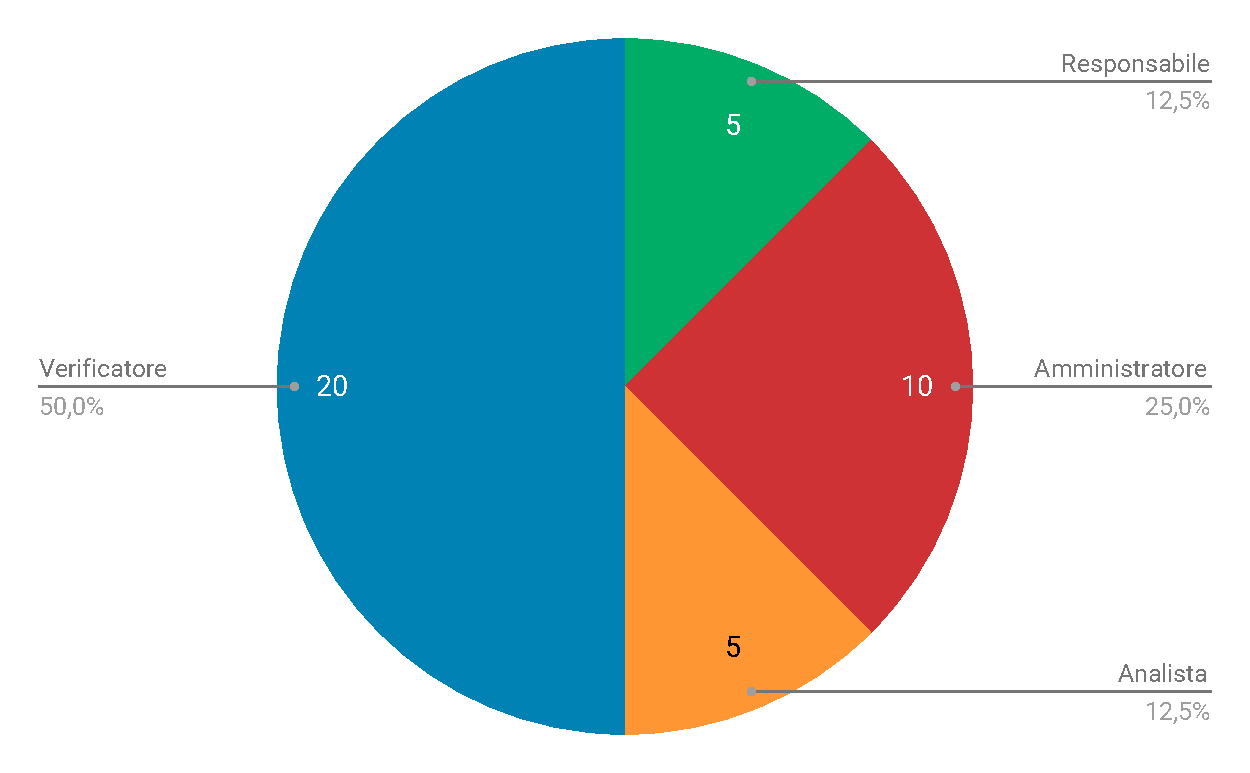
\includegraphics[width=1\linewidth]{Preventivo/grafici/CO2.pdf}
	\caption{Grafico della suddivisione oraria dei ruoli nel periodo di Consolidamento}
\end{figure}


	\subsection{Progettazione Architetturale}
		\subsubsection{Prospetto Orario}
Di seguito è riportata la suddivisione oraria dei ruoli nel periodo di Progettazione Architetturale.




\begin{table}[H]	
	\begin{center}
	    \begin{tabular}{cccccccc}
			\rowcolor{greySWEight}
			\textcolor{white}{\textbf{Nome}} & \textcolor{white}{\textbf{Re}} & \textcolor{white}{\textbf{Am}} & \textcolor{white}{\textbf{An}} & \textcolor{white}{\textbf{Pj}} & \textcolor{white}{\textbf{Pr}} & \textcolor{white}{\textbf{Ve}} & \textcolor{white}{\textbf{Totale}}
			\\
			Bacco Alberto & 5 & & 7 & 5 & & 12 & 29 \\
			Caccaro Sebastiano & & & & 12 & & 17 & 29 \\
			Ciagola Damien & & & & 12 & & 17 & 29 \\
			Corti Francesco & & 5 & & 15 & & 9 & 29 \\
			Isachi Gheorghe & & & & 14 & & 15 & 29 \\
			Legrottagle Gionata & & & & 27 & & 2 & 29 \\
			Magarotto Francesco & 5 & & & 24 & & & 29 \\
			Muraro Enrico & & 5 & & 24 & & & 29 \\
			\end{tabular}
	    \caption{Tabella della suddivisione oraria dei membri del gruppo nel periodo di Progettazione Architetturale} \label{tab:tabellaPersoneProgettazione Architetturale} 
	\end{center}
\end{table}

La tabella della suddivisione oraria è rappresentata nel seguente grafico.
\begin{figure}[H]
	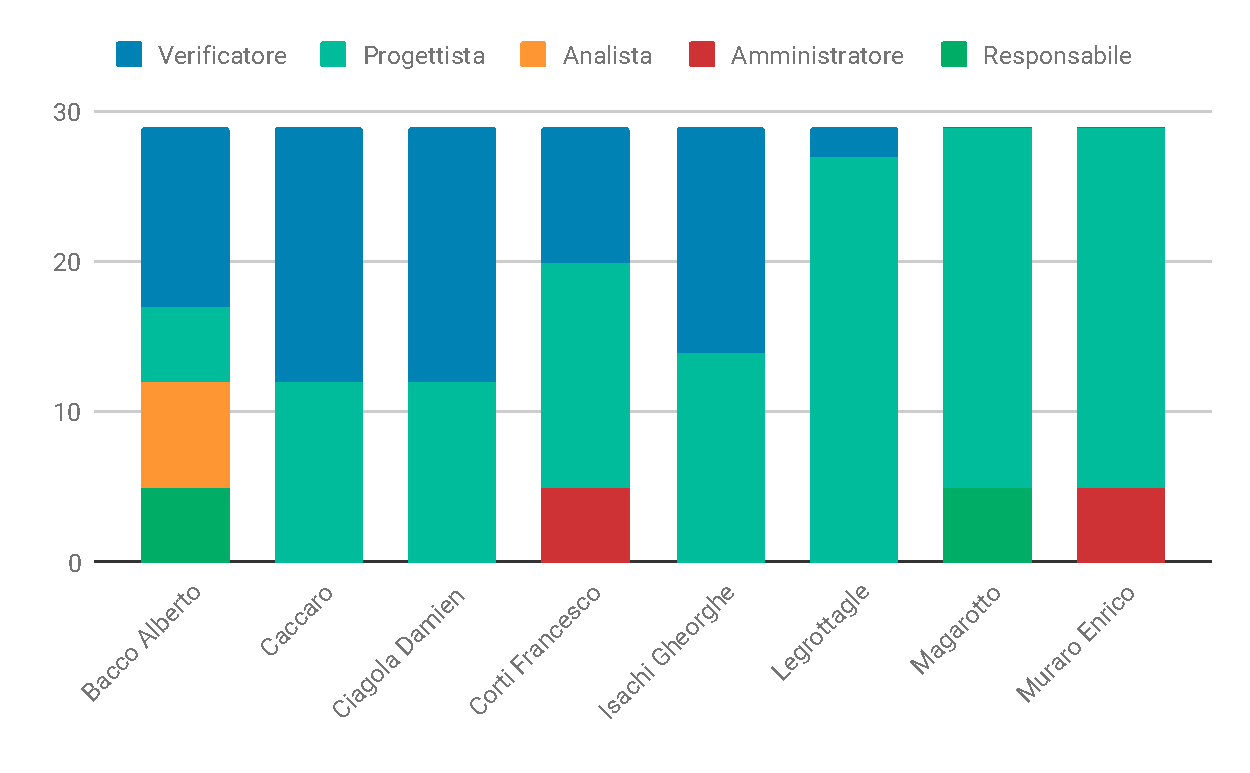
\includegraphics[width=1\linewidth]{Preventivo/grafici/PA1.pdf}
	\caption{Grafico della suddivisione oraria dei membri del gruppo nel periodo di Progettazione Architetturale}
\end{figure}

\subsubsection{Prospetto Economico}
Nella seguente tabella sono riportate le ore e i costi preventivati per ogni ruolo durante la fase di Progettazione Architetturale.


\begin{table}[H]	
	\begin{center}
	    \begin{tabular}{C{4cm}C{1cm}C{3,5cm}}
			\rowcolor{greySWEight}
			\textcolor{white}{\textbf{Ruolo}} & \textcolor{white}{\textbf{Ore}} & \textcolor{white}{\textbf{Costo}}
			\\
			Responsabile & 10 & \euro \space  300,00 \\
			Amministratore & 10 & \euro \space  200,00 \\
			Analista & 7 & \euro \space  175,00 \\
			Progettista & 133 & \euro \space  2.926,00 \\
			Programmatore &  & \euro \space  \\
			Verificatore & 72 & \euro \space  1.080,00 \\
			\textbf{Totale} & \textbf{232} & \euro \space  \textbf{4.681,00} \\
		\end{tabular}
	    \caption{Tabella della suddivisione oraria dei ruoli nel periodo di Progettazione Architetturale} \label{tab:tabellaRuoliProgettazione Architetturale} 
	\end{center}
\end{table}


Si può avere una più chiara rappresentazione della distribuzione oraria dei ruoli nel seguente grafico.

\begin{figure}[H]
	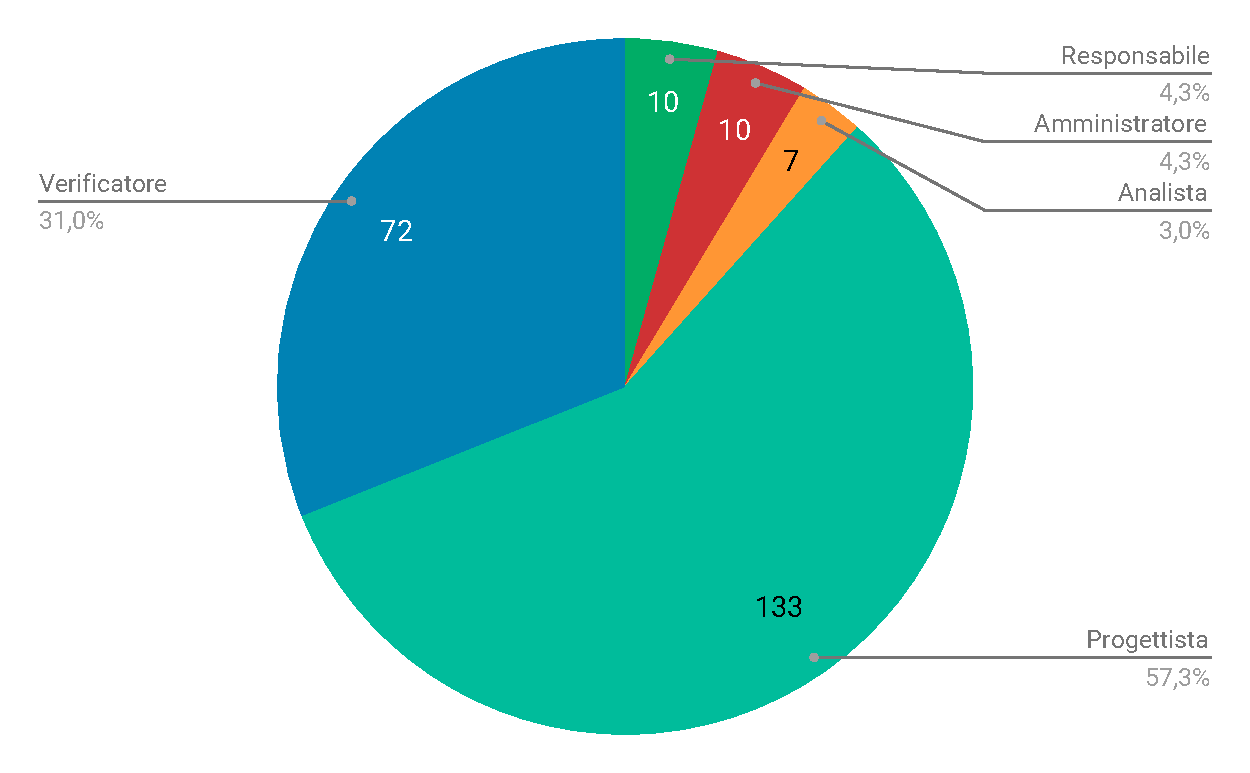
\includegraphics[width=1\linewidth]{Preventivo/grafici/PA2.pdf}
	\caption{Grafico della suddivisione oraria dei ruoli nel periodo di Progettazione Architetturale}
\end{figure}


	\subsection{Pianificazione di Dettaglio e Codifica}
		Il periodo di Progettazione di dettaglio e codifica inizia con la consegna della RP e termina con la consegna della RQ.\newline
Durante questo periodo, vengono svolte le seguenti attività:
\begin{itemize}
	\item \textbf{Incremento: }modifiche incrementali ai seguenti documenti, ove necessario:
	\begin{itemize}
		\item Analisi dei requisiti;
		\item Piano di progetto;
		\item Piano di qualifica;
		\item Glossario;
		\item Norme di progetto;
		\item Specifica Tecnica;
	\end{itemize}
	\item \textbf{Product Baseline: }sulla base della specifica tecnica viene redatto il documento di definizione di prodotto, nella quale sono contenute le scelte progettuali di dettaglio;
	\item \textbf{Codifica: }basandosi sulla definizione di prodotto, viene scritto il codice sorgente;
	\item \textbf{Manuale Utente: }redazione del manuale utente del prodotto. 
\end{itemize}


\begin{figure}[H]
	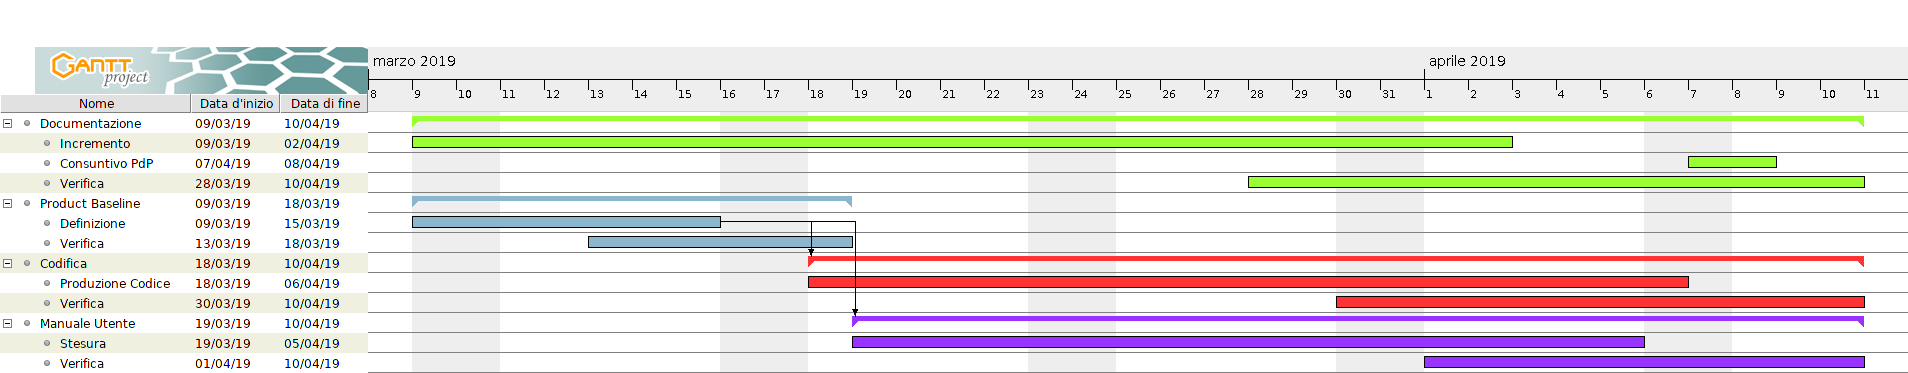
\includegraphics[width=1\linewidth]{Pianificazione/Progettazione_Dettaglio_Codififca.png}
	\caption{Diagramma di Gantt del periodo di Progettazione di dettaglio e codifica}
\end{figure}
	\subsection{Verifica e Validazione}
		Il periodo di verifica e validazione inizia con la consegna della RQ e termina con la consegna della RA.\newline
Durante questo periodo, sono svolte le seguenti attività:
\begin{itemize}
	\item \textbf{Incremento: }modifiche incrementali ai seguenti documenti, ove necessario:
	\begin{itemize}
		\item Analisi dei requisiti;
		\item Piano di progetto;
		\item Piano di qualifica;
		\item Glossario;
		\item Norme di progetto;
		\item Specifica Tecnica;
		\item Definizione di Prodotto;
		\item Manuale Utente;
	\end{itemize}
	\item \textbf{Validazione e collaudo: }il prodotto viene testato per accertarsi che soddisfi tutti i requisiti prestabiliti.
\end{itemize}


\begin{figure}[H]
	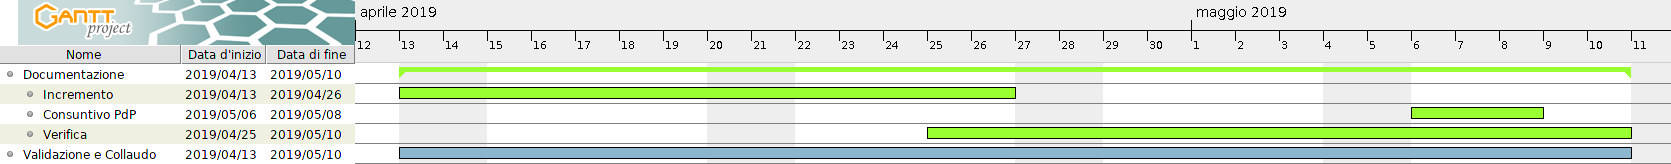
\includegraphics[width=1\linewidth]{Pianificazione/Verifica_Validazione.png}
	\caption{Diagramma di Gantt del periodo di verifica e validazione}
\end{figure}
\newpage
\section{Preventivo}
%	\subsection{Document goal}
The purpose of this document is to provide all the necessary information to extend, correct and improve Colletta.
There will be additional information regarding setting up the development environment to work in an environment that is as consistent as possible with that used
by the other members of group SWEight, but can be ignored if you only want to use part of the product.
This guide was written taking into account the Microsoft Windows and Linux operating systems. If other systems are used, compatibility issues may arise, even if it's unlikely. In this case refer to the git page. This document will grow as the product will be fully
developed.

\subsection{Product goal}
The purpose of the product is the creation of a collaborative data collection platform where users can prepare and/or perform small grammar exercises. 
The front-end of the system consists of a web application developed with React and Redux, while the back-end is a Spring Boot application written in Java, which will handle HTTP Requests sent from the front-end. 

\subsection{References}


\subsubsection{Installation references}

\begin{itemize}
\item \textbf{Git}: \url{https://git-scm.com/}
\item \textbf{Node.js}: \url{https://nodejs.org/en/}
\item \textbf{NPM}: \url{https://www.npmjs.com/}
\item \textbf{Oracle JDK}: \url{https://www.oracle.com/technetwork/java/javase/downloads/index.html}
\item \textbf{OpenJDK}: \url{https://openjdk.java.net/}
\item \textbf{Maven}: \url{https://maven.apache.org/}
\item \textbf{Lombok}: \url{https://projectlombok.org/}
\item \textbf{VSCode}: \url{https://code.visualstudio.com/} 

\end{itemize}

\subsubsection{Legal references}
\begin{itemize}
\item \textbf{MIT License}: \url{https://opensource.org/licenses/MIT}
\end{itemize}

%\subsubsection{Informative references}

	\subsection{Analisi}
	    Nella seguente tabella è illustrato il consuntivo del periodo di Analisi.

\begin{table}[H]
\centering
\begin{tabular}{c|ccc|ccc}
\rowcolor{greySWEight}
\multicolumn{1}{c}{} & \multicolumn{3}{c}{\textcolor{white}{\textbf{Ore}}} & \multicolumn{3}{c}{\textcolor{white}{\textbf{Costo in Euro}}} \\
{\textbf{Ruolo}} & {\textbf{Preventivo}} & {\textbf{Consuntivo}} & {\textbf{Delta}} & {\textbf{Preventivo}} & {\textbf{Consuntivo}} & {\textbf{Delta}} \\
Responsabile & 20 & 24 & +4 &  600,00 &  720,00 & + 120,00 \\
Amministratore & 20 & 22 & +2 &  400,00 &  440,00 & + 40,00 \\
Analista & 70 & 74 & +4 &  1.750,00 &  1.850,00 & + 100,00 \\
Progettista & 0 & 0 & 0 &  0,00 &  0,00 &  0,00 \\
Programmatore & 0 & 0 & 0 &  0,00 &  0,00 &  0,00 \\
Verificatore & 50 & 46 & -4 &  750,00 &  690,00 & - 60,00 \\
\hline
\textbf{Totale} & \textbf{160} & \textbf{166} & \textbf{+6} &  \textbf{3.500,00} &  \textbf{3.700,00} & \textbf{+ 200,00} \\


\end{tabular}
\caption{Consuntivo del periodo di Analisi}
\end{table}

	\newpage	
	\subsection{Consolidamento}
	    \subsubsection{Prospetto Orario}
Di seguito è riportata la suddivisione oraria dei ruoli nel periodo di Consolidamento.




\begin{table}[H]	
	\begin{center}
	    \begin{tabular}{cccccccc}
	  		
			\rowcolor{greySWEight}
			\textcolor{white}{\textbf{Nome}} & \textcolor{white}{\textbf{Re}} & \textcolor{white}{\textbf{Am}} & \textcolor{white}{\textbf{An}} & \textcolor{white}{\textbf{Pj}} & \textcolor{white}{\textbf{Pr}} & \textcolor{white}{\textbf{Ve}} & \textcolor{white}{\textbf{Totale}}
			\\ \hline
			Bacco Alberto & 5 & & & & & & 5 \\
			Caccaro Sebastiano & & & & & & 5 & 5 \\
			Ciagola Damien & & 5 & & & & & 5 \\
			Corti Francesco & & & & & & 5 & 5 \\
			Isachi Gheorghe & & 5 & & & & & 5 \\
			Legrottagle Gionata & & & 5 & & & & 5 \\
			Magarotto Francesco & & & & & & 5 & 5 \\
			Muraro Enrico & & & & & & 5 & 5 \\

			\end{tabular}
	    \caption{Tabella della suddivisione oraria dei membri del gruppo nel periodo di Consolidamento} \label{tab:tabellaPersoneConsolidamento} 
	\end{center}
\end{table}

La tabella della suddivisione oraria è rappresentata nel seguente grafico.
\begin{figure}[H]
	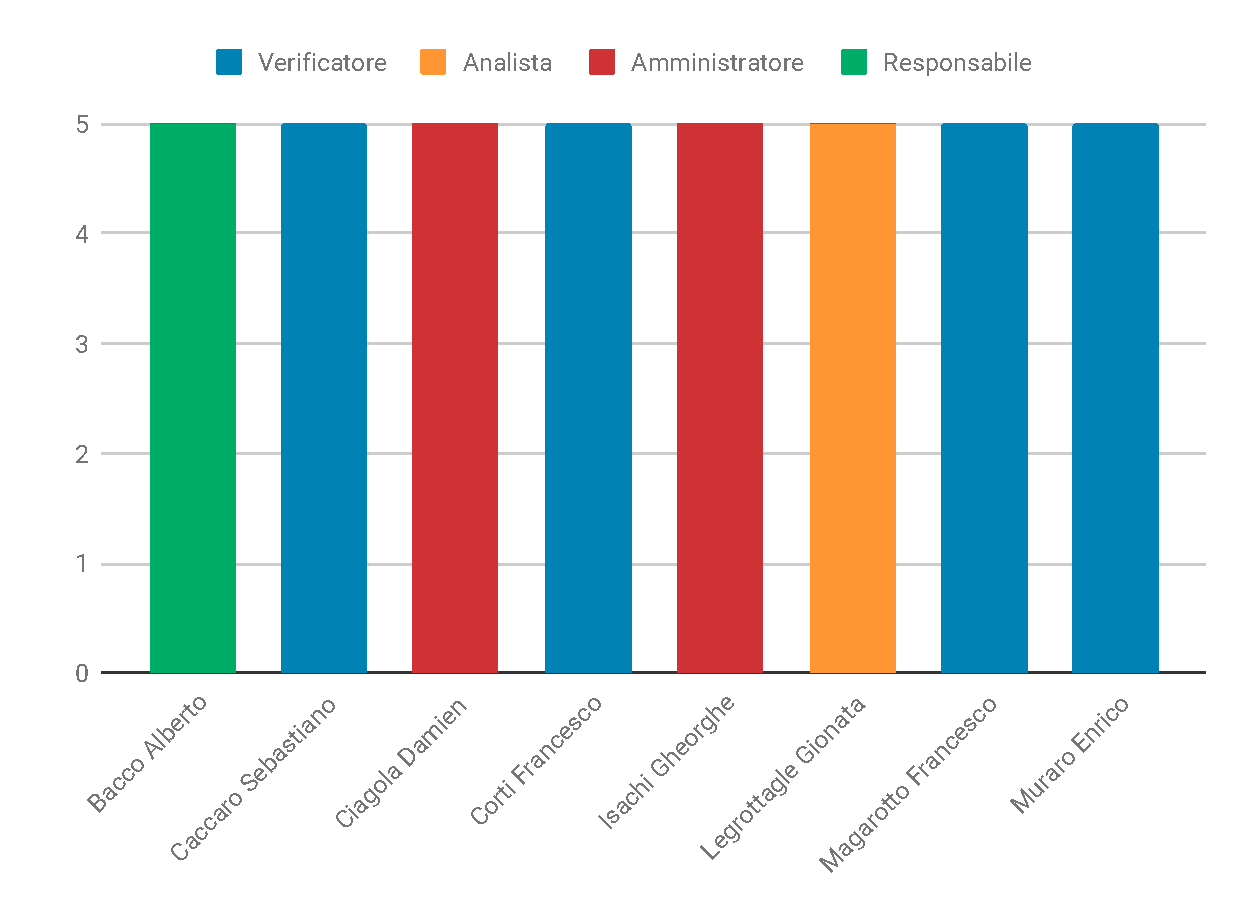
\includegraphics[width=1\linewidth]{Preventivo/grafici/CO1.pdf}
	\caption{Grafico della suddivisione oraria dei membri del gruppo nel periodo di Consolidamento}
\end{figure}

\subsubsection{Prospetto Economico}
Nella seguente tabella sono riportate le ore e i costi preventivati per ogni ruolo durante la fase di Consolidamento.


\begin{table}[H]	
	\begin{center}
	    \begin{tabular}{C{4cm}C{1cm}C{3,5cm}}
			\rowcolor{greySWEight}
			\textcolor{white}{\textbf{Ruolo}} & \textcolor{white}{\textbf{Ore}} & \textcolor{white}{\textbf{Costo}}
			\\ \hline
			Responsabile & 5 & \euro \space 150,00 \\
			Amministratore & 10 & \euro \space 200,00 \\
			Analista & 5 & \euro \space 125,00 \\
			Progettista &  & \\
			Programmatore &  &  \\
			Verificatore & 20 & \euro \space 300,00 \\
			\textbf{Totale} & \textbf{40} & \euro \space \textbf{775,00} \\
		\end{tabular}
	    \caption{Tabella della suddivisione oraria dei ruoli nel periodo di Consolidamento} \label{tab:tabellaRuoliConsolidamento} 
	\end{center}
\end{table}


Si può avere una più chiara rappresentazione della distribuzione oraria dei ruoli nel seguente grafico.

\begin{figure}[H]
	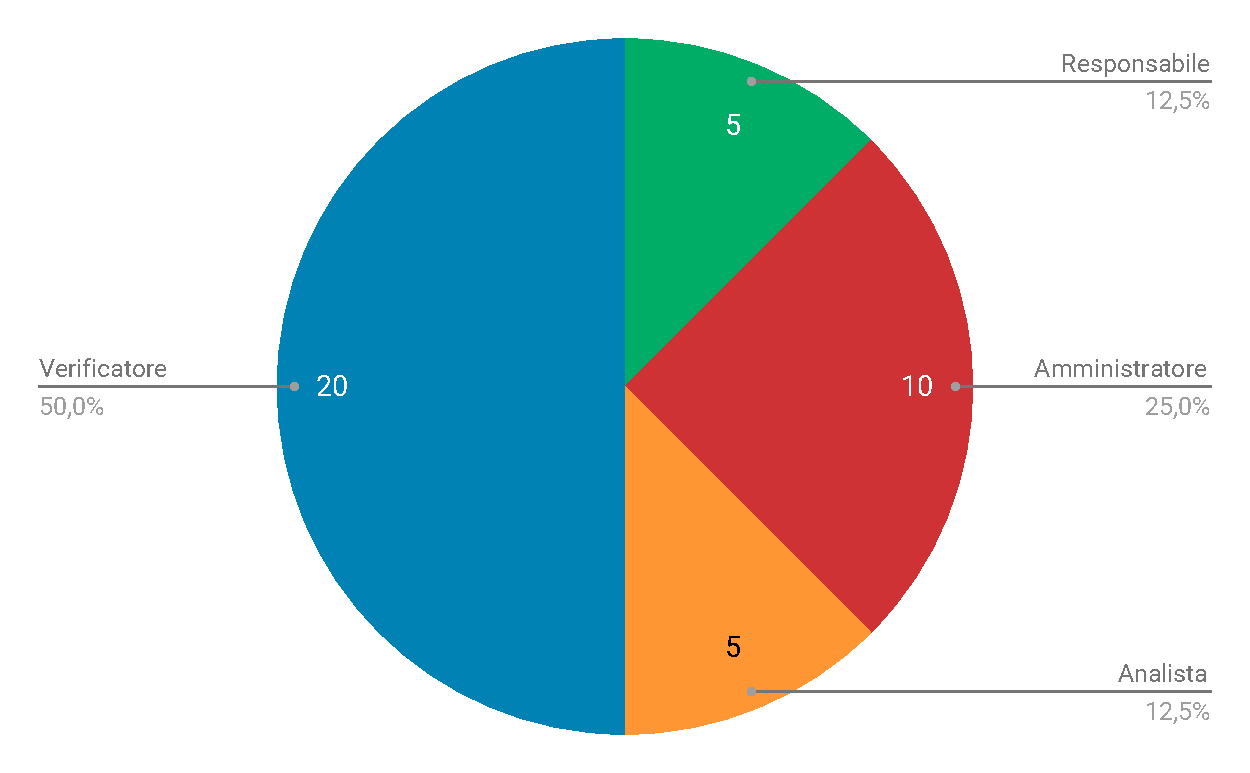
\includegraphics[width=1\linewidth]{Preventivo/grafici/CO2.pdf}
	\caption{Grafico della suddivisione oraria dei ruoli nel periodo di Consolidamento}
\end{figure}


	\newpage
%	\subsection{Progettazione Architetturale}
%	    \subsubsection{Prospetto Orario}
Di seguito è riportata la suddivisione oraria dei ruoli nel periodo di Progettazione Architetturale.




\begin{table}[H]	
	\begin{center}
	    \begin{tabular}{cccccccc}
			\rowcolor{greySWEight}
			\textcolor{white}{\textbf{Nome}} & \textcolor{white}{\textbf{Re}} & \textcolor{white}{\textbf{Am}} & \textcolor{white}{\textbf{An}} & \textcolor{white}{\textbf{Pj}} & \textcolor{white}{\textbf{Pr}} & \textcolor{white}{\textbf{Ve}} & \textcolor{white}{\textbf{Totale}}
			\\
			Bacco Alberto & 5 & & 7 & 5 & & 12 & 29 \\
			Caccaro Sebastiano & & & & 12 & & 17 & 29 \\
			Ciagola Damien & & & & 12 & & 17 & 29 \\
			Corti Francesco & & 5 & & 15 & & 9 & 29 \\
			Isachi Gheorghe & & & & 14 & & 15 & 29 \\
			Legrottagle Gionata & & & & 27 & & 2 & 29 \\
			Magarotto Francesco & 5 & & & 24 & & & 29 \\
			Muraro Enrico & & 5 & & 24 & & & 29 \\
			\end{tabular}
	    \caption{Tabella della suddivisione oraria dei membri del gruppo nel periodo di Progettazione Architetturale} \label{tab:tabellaPersoneProgettazione Architetturale} 
	\end{center}
\end{table}

La tabella della suddivisione oraria è rappresentata nel seguente grafico.
\begin{figure}[H]
	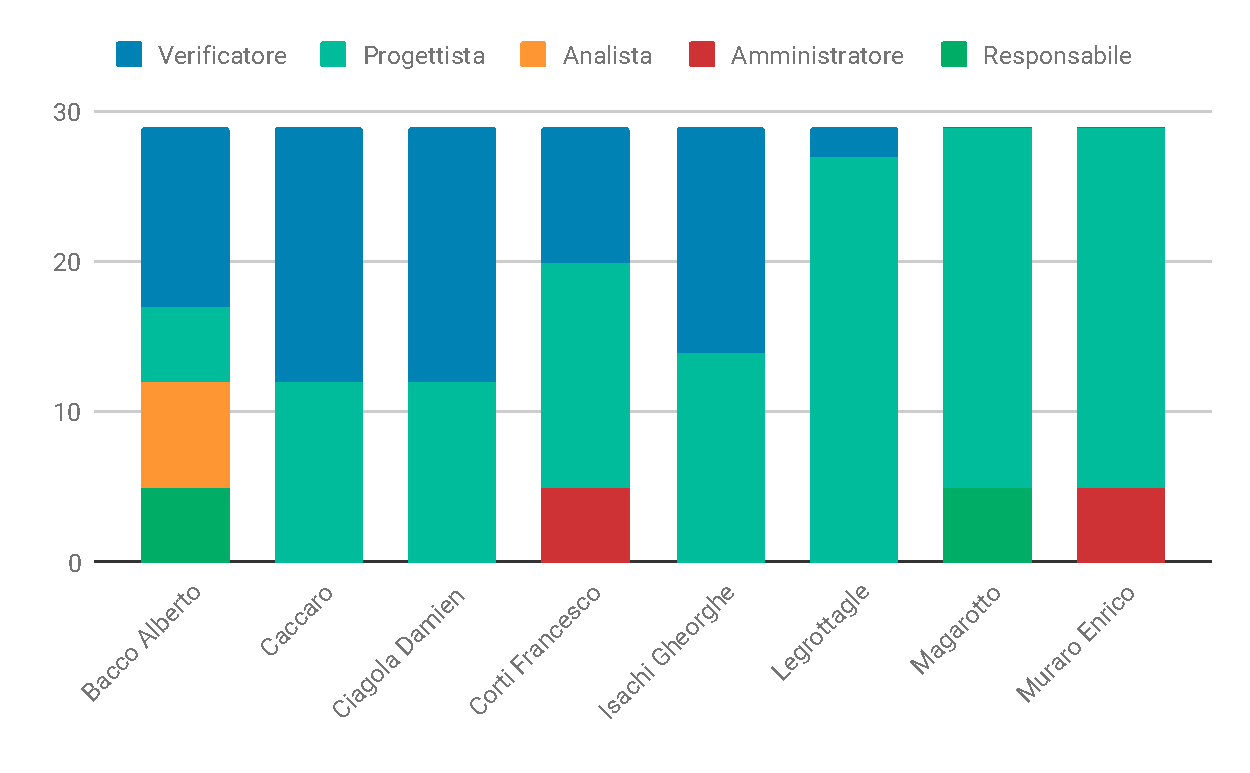
\includegraphics[width=1\linewidth]{Preventivo/grafici/PA1.pdf}
	\caption{Grafico della suddivisione oraria dei membri del gruppo nel periodo di Progettazione Architetturale}
\end{figure}

\subsubsection{Prospetto Economico}
Nella seguente tabella sono riportate le ore e i costi preventivati per ogni ruolo durante la fase di Progettazione Architetturale.


\begin{table}[H]	
	\begin{center}
	    \begin{tabular}{C{4cm}C{1cm}C{3,5cm}}
			\rowcolor{greySWEight}
			\textcolor{white}{\textbf{Ruolo}} & \textcolor{white}{\textbf{Ore}} & \textcolor{white}{\textbf{Costo}}
			\\
			Responsabile & 10 & \euro \space  300,00 \\
			Amministratore & 10 & \euro \space  200,00 \\
			Analista & 7 & \euro \space  175,00 \\
			Progettista & 133 & \euro \space  2.926,00 \\
			Programmatore &  & \euro \space  \\
			Verificatore & 72 & \euro \space  1.080,00 \\
			\textbf{Totale} & \textbf{232} & \euro \space  \textbf{4.681,00} \\
		\end{tabular}
	    \caption{Tabella della suddivisione oraria dei ruoli nel periodo di Progettazione Architetturale} \label{tab:tabellaRuoliProgettazione Architetturale} 
	\end{center}
\end{table}


Si può avere una più chiara rappresentazione della distribuzione oraria dei ruoli nel seguente grafico.

\begin{figure}[H]
	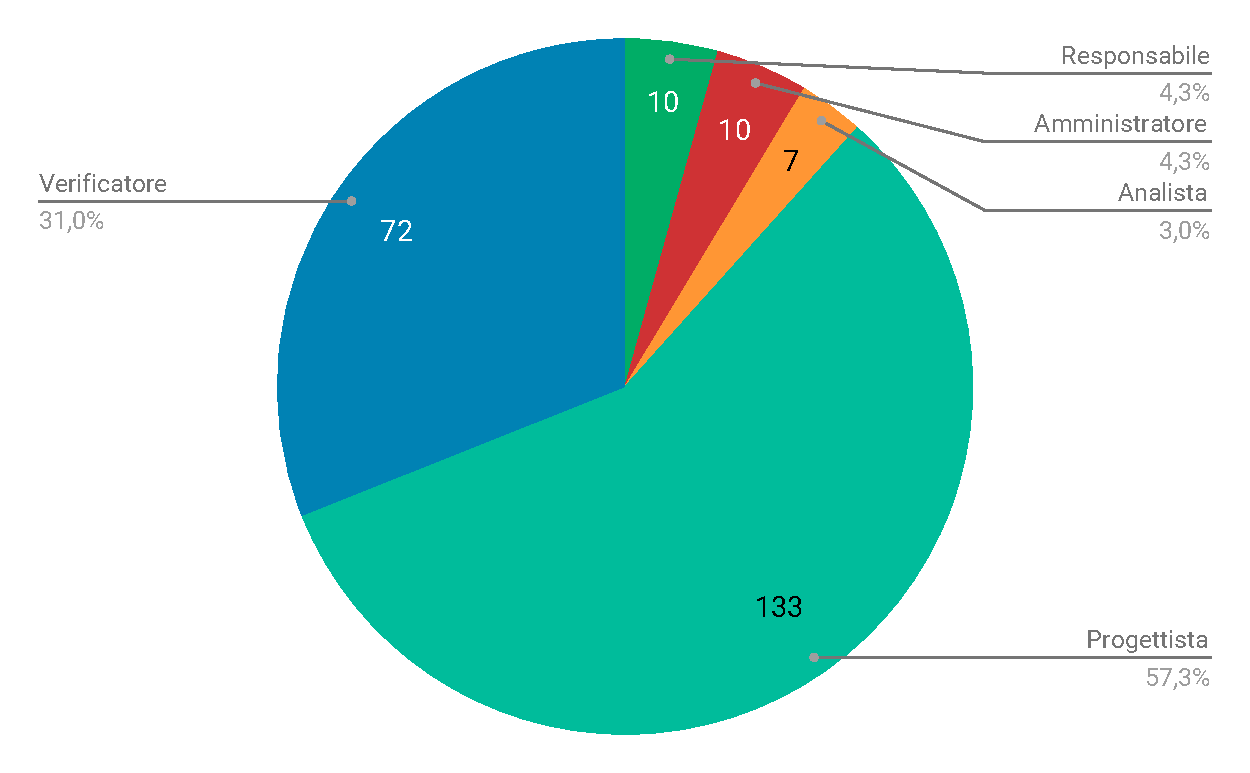
\includegraphics[width=1\linewidth]{Preventivo/grafici/PA2.pdf}
	\caption{Grafico della suddivisione oraria dei ruoli nel periodo di Progettazione Architetturale}
\end{figure}


	\newpage
%	\subsection{Pianificazione di Dettaglio e Codifica}
%	    Il periodo di Progettazione di dettaglio e codifica inizia con la consegna della RP e termina con la consegna della RQ.\newline
Durante questo periodo, vengono svolte le seguenti attività:
\begin{itemize}
	\item \textbf{Incremento: }modifiche incrementali ai seguenti documenti, ove necessario:
	\begin{itemize}
		\item Analisi dei requisiti;
		\item Piano di progetto;
		\item Piano di qualifica;
		\item Glossario;
		\item Norme di progetto;
		\item Specifica Tecnica;
	\end{itemize}
	\item \textbf{Product Baseline: }sulla base della specifica tecnica viene redatto il documento di definizione di prodotto, nella quale sono contenute le scelte progettuali di dettaglio;
	\item \textbf{Codifica: }basandosi sulla definizione di prodotto, viene scritto il codice sorgente;
	\item \textbf{Manuale Utente: }redazione del manuale utente del prodotto. 
\end{itemize}


\begin{figure}[H]
	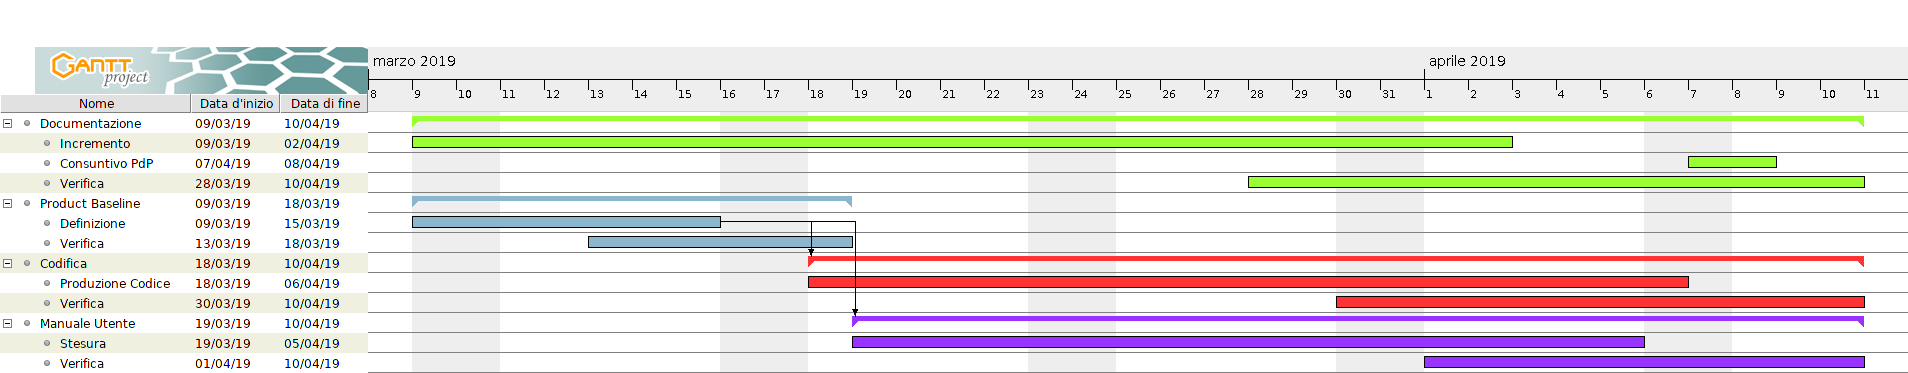
\includegraphics[width=1\linewidth]{Pianificazione/Progettazione_Dettaglio_Codififca.png}
	\caption{Diagramma di Gantt del periodo di Progettazione di dettaglio e codifica}
\end{figure}
	\newpage
%	\subsection{Verifica e Validazione}
%	    Il periodo di verifica e validazione inizia con la consegna della RQ e termina con la consegna della RA.\newline
Durante questo periodo, sono svolte le seguenti attività:
\begin{itemize}
	\item \textbf{Incremento: }modifiche incrementali ai seguenti documenti, ove necessario:
	\begin{itemize}
		\item Analisi dei requisiti;
		\item Piano di progetto;
		\item Piano di qualifica;
		\item Glossario;
		\item Norme di progetto;
		\item Specifica Tecnica;
		\item Definizione di Prodotto;
		\item Manuale Utente;
	\end{itemize}
	\item \textbf{Validazione e collaudo: }il prodotto viene testato per accertarsi che soddisfi tutti i requisiti prestabiliti.
\end{itemize}


\begin{figure}[H]
	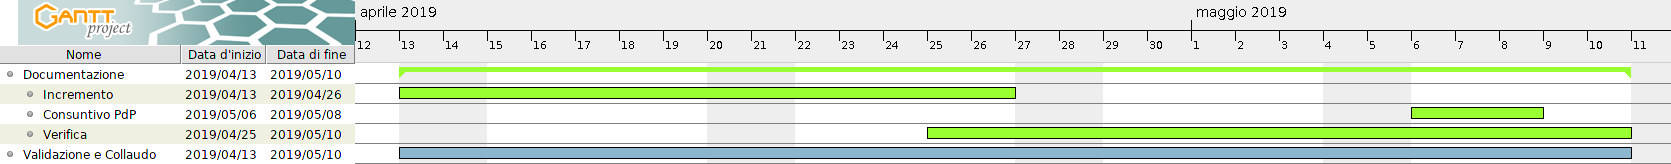
\includegraphics[width=1\linewidth]{Pianificazione/Verifica_Validazione.png}
	\caption{Diagramma di Gantt del periodo di verifica e validazione}
\end{figure}
	
\newpage
\section{Consuntivo e preventivo a finire}

\end{document}